\documentclass{standalone}
\usepackage{tikz}
\usepackage{ctex,siunitx}
\setCJKmainfont{Noto Serif CJK SC}
\usepackage{tkz-euclide}
\usepackage{amsmath}
\usetikzlibrary{patterns, calc}
\usetikzlibrary {decorations.pathmorphing, decorations.pathreplacing, decorations.shapes,}
\begin{document}
\small
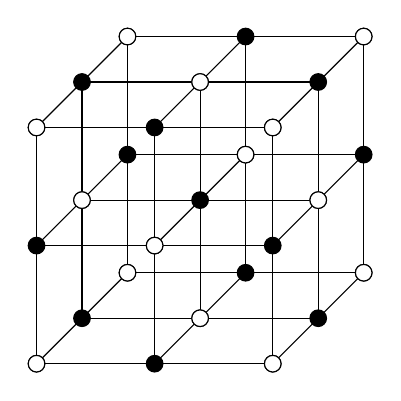
\begin{tikzpicture}[>=stealth,scale=1.5]
  % \useasboundingbox(-1,-2)rectangle(8,6);
  \draw (0,0,0)--(0,0,2);
  \draw (0,0,0)--(0,2,0);
  \draw (0,0,0)--(2,0,0);
  \draw (0,1,0)--(0,1,2);
  \draw (0,1,0)--(2,1,0);
  \draw (0,2,0)--(0,2,2);
  \draw (0,2,0)--(2,2,0);
  \draw (1,1,0)--(1,1,2);
  \draw (1,2,0)--(1,2,2);
  \draw (2,1,0)--(2,1,2);
  \draw (2,2,0)--(2,2,2);
  \draw (1,0,0)--(1,0,2);
  \draw (1,0,0)--(1,2,0);
  \draw (2,0,0)--(2,0,2);
  \draw (2,0,0)--(2,2,0);
  \draw(0,2,1)--(2,2,1);
  \draw(0,2,2)--(2,2,2);
  \draw(0,1,1)--(2,1,1);
  \draw(0,1,2)--(2,1,2);
  \draw (0,2,2)--(0,0,2);
  \draw (2,0,2)--(0,0,2);
  \draw (2,0,1)--(0,0,1);
  \draw (2,0,2)--(2,2,2);
  \draw (2,0,1)--(2,2,1);
  \draw (1,0,1)--(1,2,1);
  \draw (1,0,2)--(1,2,2);
  \draw (0,0,1)--(0,2,1);
  \foreach \x in {0,1,2}
  \foreach \y in {0,1,2}
  \foreach \z in {0,1,2}
  {
  \draw [fill=black](\x,\y,\z) circle (2pt);
  }
  \draw [fill=white] ( 0,0,0 )  circle (2pt);
  \draw [fill=white] ( 0,0,2 )  circle (2pt);
  \draw [fill=white] ( 0,1,1 )  circle (2pt);
  \draw [fill=white] ( 1,0,1 )  circle (2pt);
  \draw [fill=white] ( 2,0,0 )  circle (2pt);
  \draw [fill=white] ( 2,0,2 )  circle (2pt);
  \draw [fill=white] ( 2,1,1 )  circle (2pt);
  \draw [fill=white] ( 1,2,1 )  circle (2pt);
  \draw [fill=white] ( 0,2,0 )  circle (2pt);
  \draw [fill=white] ( 0,2,2 )  circle (2pt);
  \draw [fill=white] ( 1,1,0 )  circle (2pt);
  \draw [fill=white] ( 1,1,2 )  circle (2pt);
  \draw [fill=white] ( 2,2,0 )  circle (2pt);
  \draw [fill=white] ( 2,2,2 )  circle (2pt);
\end{tikzpicture}
\end{document}